%File: less_is_more_aaai.tex
%
% AAAI 2026 TEMPLATE for "Less is More" Paper
% For ANONYMOUS SUBMISSION: uncomment the next line
% \def\aaaianonymous{true}
%
% For CAMERA-READY VERSION: comment out or delete the next line
% \def\aaaianonymous{true}
%
%%%%%%%%%%%%%%%%%%%%%%%%%%%%%%%%%%%%%%%%%%%%%%%%%%%%%%%%%%%%%%%%%%%%%%%

\documentclass[letterpaper]{article} % DO NOT CHANGE THIS

% Conditional package loading based on version
\ifdefined\aaaianonymous
    \usepackage[submission]{aaai2026}  % Anonymous submission version
\else
    \usepackage{aaai2026}              % Camera-ready version
\fi

\usepackage{times}  % DO NOT CHANGE THIS
\usepackage{helvet}  % DO NOT CHANGE THIS
\usepackage{courier}  % DO NOT CHANGE THIS
\usepackage[hyphens]{url}  % DO NOT CHANGE THIS
\usepackage{graphicx} % DO NOT CHANGE THIS
\urlstyle{rm} % DO NOT CHANGE THIS
\def\UrlFont{\rm}  % DO NOT CHANGE THIS
\usepackage{natbib}  % DO NOT CHANGE THIS AND DO NOT ADD ANY OPTIONS TO IT
\usepackage{caption} % DO NOT CHANGE THIS AND DO NOT ADD ANY OPTIONS TO IT
\frenchspacing  % DO NOT CHANGE THIS
\setlength{\pdfpagewidth}{8.5in} % DO NOT CHANGE THIS
\setlength{\pdfpageheight}{11in} % DO NOT CHANGE THIS

% Additional packages for tables and math
\usepackage{booktabs}
\usepackage{multirow}
\usepackage{amsmath}

%
% Keep the \pdfinfo as shown here. There's no need
% for you to add the /Title and /Author tags.
\pdfinfo{
/TemplateVersion (2026.1)
}

\setcounter{secnumdepth}{0} %May be changed to 1 or 2 if section numbers are desired.

% Title - conditionally set based on version
\ifdefined\aaaianonymous
    \title{Less is More: Simple Linear Fusion Outperforms Complex Retrieval-Augmented Generation Systems}
\else
    \title{Less is More: Simple Linear Fusion Outperforms Complex Retrieval-Augmented Generation Systems}
\fi

% Author and affiliation information
\ifdefined\aaaianonymous
\author{
    Anonymous Submission
}
\affiliations{
    Anonymous Institution\\
    Anonymous Address\\
    anonymous@email.com
}
\else
\author{
    Runtao Wang\textsuperscript{\rm 1},
    Fufangchen Zhao\textsuperscript{\rm 1},
    Danfeng Yan\textsuperscript{\rm 1,*}
}
\affiliations{
    \textsuperscript{\rm 1}Beijing University of Posts and Telecommunications\\
    Beijing, China\\
    wrt136@bupt.edu.cn, zhaofufangchen@bupt.edu.cn, yandf@bupt.edu.cn\\
    \textsuperscript{*}Corresponding author
}
\fi

\begin{document}

\maketitle

\begin{abstract}
In information retrieval, multi-retriever fusion has become an important technique for improving retrieval performance. The conventional wisdom suggests that more complex fusion strategies yield better results, prompting researchers to develop increasingly sophisticated methods. However, our research challenges this assumption by proposing a "Less is More" perspective.

Our experimental results reveal an interesting finding: \textbf{under the specific datasets and experimental conditions of this study, simple linear fusion methods can in certain cases achieve or exceed the performance of complex methods}. Specifically, simple linear fusion outperforms the standard RRF method by 8.2\%, 7.2\%, and 10.9\% in MRR performance on FIQA, Quora, and SciDocs datasets respectively, with a 2.2\% improvement on SciFact dataset. Importantly, ablation experiments show that removing complex components (such as query analyzers) can improve performance in certain cases. Additionally, simple methods have significant advantages in computational efficiency, with inference speed significantly faster than complex methods.

These findings provide empirical support in specific scenarios for the hypothesis that "simple methods may be more effective," questioning the prevalent assumption that "complexity equals better," and providing important reference principles for practical system design.
\end{abstract}

% Links section removed - code and datasets not publicly available

\section{Introduction}

With the development of large language models and Retrieval-Augmented Generation (RAG) technology \cite{lewis2020retrieval}, multi-retriever fusion has become an important research direction in information retrieval. In recent years, RAG technology has rapidly evolved from basic retrieval-generation architectures to more complex multimodal \cite{chen2022multimodal} and agent-based systems \cite{singh2025agentic}, with the latest survey studies \cite{gao2024retrieval} systematically reviewing the development trajectory and future directions of RAG technology. Multi-retriever systems improve retrieval performance by combining different types of retrievers (such as dense vector retrieval \cite{karpukhin2020dense} and sparse BM25 retrieval \cite{robertson2009probabilistic}), but how to effectively fuse the results of multiple retrievers has become a key challenge.

\subsection{Background and Motivation}

\textbf{From Practical Needs to Theoretical Discovery}

This research stems from our practical experience in building production-level multi-retriever fusion systems. Inspired by the numerous complex fusion strategies proposed by the academic community in recent years, we conducted a systematic analysis of recent papers and identified several major innovation directions:

\begin{enumerate}
\item \textbf{Query Analysis and Classification}: Such as query decomposition proposed by LevelRAG \cite{jiang2023levelrag} and complexity classification by Adaptive-RAG \cite{jeong2024adaptive}
\item \textbf{Dynamic Weight Adjustment}: Mechanisms that dynamically adjust fusion weights based on query features
\item \textbf{Adaptive Routing Strategies}: Such as the parameter adaptive system of HyPA-RAG \cite{su2024hypa}
\item \textbf{Knowledge Graph Enhancement}: Such as structured knowledge integration of KG-Infused RAG \cite{edge2024kg}
\end{enumerate}

Based on these advanced concepts, we built a complete system architecture containing query analyzers, adaptive routers, and dynamic fusion engines (detailed in Section 3), expecting to significantly improve retrieval performance by increasing system complexity. Our initial hypothesis was that more complex adaptive mechanisms could intelligently select optimal fusion strategies based on query features, thereby outperforming simple static methods.

\textbf{The "Less is More" Phenomenon in AI}

The "Less is More" phenomenon is evident across multiple domains of artificial intelligence. In deep learning, Dropout \cite{srivastava2014dropout} and regularization techniques improve generalization by reducing model complexity; in natural language processing, simple n-gram models can still compete with complex neural network models on certain tasks \cite{chen1999empirical}; in computer vision, lightweight networks like MobileNet \cite{howard2017mobilenets} significantly reduce computational complexity while maintaining performance. These success cases demonstrate that Occam's Razor principle \cite{domingos1999role,baker2016simplicity} has important guiding significance in AI system design: under equal conditions, the simplest explanation or model should be chosen.

\subsection{Unexpected Discovery}

\textbf{Challenging Initial Assumptions}

However, in systematic experimental evaluation on 6 BEIR datasets \cite{thakur2021beir}, we obtained an important finding: \textbf{under our experimental conditions, simple linear fusion methods performed better than our designed complex adaptive system on most datasets}.

This finding completely overturned our initial assumptions. We originally expected the query analyzer to accurately identify query types, the adaptive router to intelligently select optimal strategies, and the dynamic fusion engine to adjust weights based on context. But experimental results showed that these complex components not only failed to improve performance, but in some cases even had negative effects.

\textbf{Quantified Performance Comparison Results}:

\begin{itemize}
\item Simple linear fusion outperformed standard RRF by 8.2\%, 7.2\%, and 10.9\% on FIQA, Quora, and SciDocs datasets respectively, with a 2.2\% improvement on SciFact dataset\\
\item Ablation experiments revealed an even more noteworthy phenomenon: gradually removing complex components (such as query analyzers and adaptive routers) not only did not degrade performance, but even brought 10.9\% performance improvement on SciDocs dataset\\
\item Computational efficiency analysis showed that simple methods have significant advantages in inference speed, while complex adaptive systems have significantly higher computational overhead
\end{itemize}

These findings under specific experimental conditions challenge our initial design philosophy, and more importantly question the prevalent assumption of "complexity equals better" in the information retrieval field, providing empirical support for the "Less is More" design philosophy.

\textbf{Main Contributions}: We provide systematic empirical validation across 8 fusion strategies on 6 BEIR datasets, revealing that simple linear methods often outperform complex adaptive approaches. Through detailed ablation experiments, we demonstrate the negative impacts of complex components including error propagation and computational overhead, leading to practical "simplicity first" design principles for retrieval systems.

\subsection{Complexity Classification}

We categorize fusion methods into three complexity levels based on parameter count, computational requirements, and system architecture: \textbf{Simple Methods} (linear weighted fusion, max score), \textbf{Medium Complexity} (RRF with mathematical foundations), and \textbf{Complex Methods} (adaptive fusion requiring multiple coordinated subsystems).

\section{Related Work}

\subsection{Fusion Methods}

Multi-retriever fusion has been extensively studied in information retrieval. Traditional approaches include Reciprocal Rank Fusion (RRF) \cite{cormack2009reciprocal}, which combines rankings from different retrievers using reciprocal rank scores, and linear weighted fusion methods first proposed by Fox and Shaw \cite{fox1994combination}. Recent work has explored more sophisticated fusion strategies, including learning-to-rank approaches \cite{liu2009learning} and neural fusion methods \cite{zamani2018neural}. Modern approaches have also incorporated dynamic weight adjustment mechanisms, such as DAT (Dynamic Adaptive Threshold) \cite{hsu2025dat}, which introduces dynamic threshold mechanisms based on query features.

\subsection{Retrieval-Augmented Generation}

RAG systems have gained significant attention with the rise of large language models \cite{lewis2020retrieval}. Recent surveys \cite{gao2024retrieval,gupta2024comprehensive} provide comprehensive overviews of RAG architectures and applications. Multi-modal RAG systems \cite{chen2022multimodal,zheng2025retrieval} and agent-based approaches \cite{singh2025agentic} represent the latest developments in this field. Modern retrieval methods have evolved from traditional sparse methods like TF-IDF \cite{salton1988term} and BM25 \cite{robertson2009probabilistic} to dense retrieval approaches using pre-trained models like BERT \cite{devlin2019bert} and Transformer architectures \cite{vaswani2017attention}. Recent innovations include ColBERT \cite{khattab2020colbert} for late interaction, SPLADE \cite{formal2021splade} for sparse neural retrieval, and contrastive learning approaches like SimCSE \cite{gao2021simcse}.

\subsection{Adaptive Routing}

Query analysis and routing represent another class of methods for improving retrieval performance by analyzing query characteristics to select the most appropriate retrieval strategies. Recent developments in agentic RAG systems \cite{singh2025agentic} have brought new perspectives to query routing by introducing agent-based planning and decision-making capabilities to optimize the retrieval process.

\subsubsection{Query Decomposition}

LevelRAG \cite{jiang2023levelrag} proposed a hierarchical architecture that uses high-level searchers to decompose complex queries into atomic queries, which are then optimized by low-level searchers. This method is particularly suitable for multi-hop reasoning tasks but has high system complexity requiring coordination of multiple components.

\subsubsection{Complexity Classification}

Adaptive-RAG \cite{jeong2024adaptive} proposed a classification method based on query complexity, categorizing queries into simple, medium, and complex classes, and selecting different retrieval strategies for each class. This method embodies the idea of adaptive processing based on query characteristics, but accurate classification of query complexity remains a challenge.

\subsubsection{Routing Strategies}

Self-RAG \cite{asai2023selfrag} and similar works proposed routing mechanisms based on model self-reflection, dynamically deciding when to retrieve and what content to retrieve. These methods increase system flexibility but also significantly increase computational complexity and implementation difficulty.

\section{Methodology}

This section details the complete multi-retriever fusion system we built and the various fusion strategies implemented and evaluated. We will first present the overall system architecture design, then introduce the selection and configuration of basic retrievers, followed by detailed descriptions of implementation details from simple linear fusion to complex adaptive methods, and finally analyze their theoretical foundations and computational complexity.

\subsection{System Architecture}

\textbf{Complete Multi-Retriever Fusion System}

To systematically compare the performance of different fusion strategies, we built a complete retrieval system containing multiple components. The system's design philosophy is to support various fusion strategies from simple to complex through a modular approach, ensuring fairness in experimental comparisons.

\textbf{System Architecture}: Our system integrates 6 diverse retrievers with a query analyzer for feature extraction, an adaptive router for strategy selection, and a multi-strategy fusion engine supporting 8 fusion methods from simple linear to complex adaptive approaches.

\textbf{Design Intent and Expectations}:

Our intention in building this complex system was to expect significant retrieval performance improvements through intelligent query analysis, adaptive routing decisions, and dynamic fusion weight adjustment. We hypothesized that system complexity could bring corresponding performance benefits, especially in automatically selecting optimal strategies when processing different types of queries.

However, as subsequent experimental results show, the actual performance of this complex system formed a sharp contrast with our expectations, leading to deep thinking about the "relationship between complexity and performance."

\subsection{Basic Retrievers}

\textbf{Main Retriever Configuration}

Although our system supports 6 different retrievers, to ensure consistency in experimental comparisons and interpretability of results, we mainly use two complementary retrievers in fusion strategy comparison experiments. This choice is based on their complementarity on different types of queries and stable performance in BEIR benchmark tests. This design philosophy is consistent with the collaborative working principles of multi-retriever emphasized in recent RAG system research \cite{gao2024retrieval}, improving overall retrieval performance by combining the advantages of sparse and dense retrievers.

\subsubsection{Sparse Retriever (BM25)}

We use the BM25 algorithm as the sparse retriever with standard parameters ($k_1 = 1.2$, $b = 0.75$), which provides excellent exact keyword matching capabilities.

\subsubsection{Dense Retriever (E5-large-v2)}

For dense retrieval, we use the E5-large-v2 model \cite{wang2022text}, which provides 1024-dimensional embeddings and excels at semantic matching tasks.

\subsubsection{Complementarity Analysis}

The combination of BM25 and E5-large-v2 provides good complementarity:

\begin{itemize}
\item \textbf{Query Type Coverage}: BM25 excels at keyword queries, while E5-large-v2 performs better on semantic queries\\
\item \textbf{Matching Mechanism}: BM25 uses exact term matching, while E5-large-v2 uses semantic similarity\\
\item \textbf{Failure Mode Diversity}: Different retrievers fail on different types of queries, providing robustness through fusion
\end{itemize}

\subsection{Fusion Strategy Design}

\textbf{Strategy Spectrum from Simple to Complex}

We implemented and evaluated 8 fusion strategies in our system, from the simplest linear weighting to the most complex adaptive fusion, covering current mainstream fusion methods. Each strategy has its specific design philosophy and applicable scenarios. Our design draws from traditional fusion method ideas while also referencing innovative methods like RAG-Fusion \cite{rackauckas2024rag}.

\textbf{Experimental Design Philosophy}: Our goal is to verify our initial hypothesis through systematic comparative experiments—complex adaptive strategies should outperform simple static methods. To this end, we carefully designed a strategy gradient from simple to complex, expecting to observe performance improvements with increasing complexity.

\subsubsection{Fusion Strategy Overview}

We implement three categories of fusion approaches with increasing complexity. \textbf{Simple strategies} include equal-weight linear fusion (0.5:0.5), BM25-dominant fusion (0.7:0.3), vector-dominant fusion (0.3:0.7), and max score selection. \textbf{Medium complexity approaches} use Reciprocal Rank Fusion with either standard (k=60) or optimized parameters. \textbf{Complex methods} employ query analysis for adaptive weight selection or dynamic adjustment based on multiple query features including length, entity count, and semantic complexity.

\subsection{Complex Components}

\textbf{Core Components of Adaptive System}

To implement our envisioned intelligent fusion system, we developed three core complex components: query analyzer, adaptive router, and dynamic fusion engine. The design of these components embodies our understanding and expectations of "intelligent retrieval."

\subsubsection{Query Analyzer}

The query analyzer is responsible for analyzing input queries and extracting features for adaptive fusion decisions. It includes the following modules:

\begin{itemize}
\item \textbf{Feature Extraction}: Extract query length, entity count, keyword density, etc.\\
\item \textbf{Query Classification}: Classify queries into entity, keyword, or semantic types\\
\item \textbf{Confidence Assessment}: Evaluate classification confidence for decision making
\end{itemize}

However, our query analyzer achieved only 67.3\% classification accuracy, which became a major factor in system performance degradation.

\subsubsection{Adaptive Router}

The adaptive router selects optimal fusion strategies based on query analysis results:

\begin{itemize}
\item \textbf{Strategy Selection}: Choose appropriate fusion methods based on query type
\item \textbf{Parameter Adjustment}: Dynamically adjust fusion parameters
\item \textbf{Fallback Mechanism}: Use default strategies when confidence is low
\end{itemize}

\textbf{Complex System Design Expectations vs. Reality}

When designing these complex components, we expected them to work collaboratively to form an intelligent retrieval system: the query analyzer provides accurate query understanding, the adaptive router makes optimal strategy selections, and the dynamic fusion engine implements precise weight adjustments. We believed this complexity could bring significant performance improvements, especially when handling diverse queries.

However, as subsequent experimental results show, these carefully designed complex components did not bring expected benefits, but rather became performance bottlenecks in some cases. This finding prompted us to reconsider the relationship between complexity and performance.

\section{Experimental Setup}

\subsection{Datasets}

We evaluate our methods on 6 datasets from the BEIR benchmark \cite{thakur2021beir}: FIQA (financial QA), Quora (question duplicates), SciDocs (scientific documents), NFCorpus (nutrition facts), SciFact (fact verification), and ArguAna (argument retrieval), representing diverse domains and query types.

\subsection{Evaluation Metrics}

We use Mean Reciprocal Rank (MRR) as the primary evaluation metric, which is widely used in information retrieval and provides a good balance between precision and ranking quality.

\subsection{Implementation Details}

All experiments are conducted using the same hardware configuration and software environment. We retrieve top-1000 documents from each retriever and re-rank using fusion strategies to top-100. Each experimental configuration is repeated 5 times with different random seeds (42, 123, 456, 789, 1024), and we report mean and standard deviation.

\textbf{Experimental Protocol}: All experiments use consistent hardware/software environments with grid search parameter optimization and statistical significance testing (p < 0.05).

\section{Results and Analysis}

\textbf{From Expectation to Reality: Unexpected Experimental Findings}

This section presents our systematic experimental results on 6 BEIR datasets. These results not only challenge our initial hypotheses but more importantly provide important insights into the "relationship between complexity and performance" in the information retrieval field.

\subsection{Baseline Comparison}

\textbf{Initial Validation: Competitiveness of Simple Methods}

Table \ref{tab:baseline} shows the MRR performance of different baseline methods on 6 datasets.

\begin{table}[t]
\centering
\caption{Baseline Comparison Results (MRR ± Standard Deviation)}
\label{tab:baseline}
\small
\begin{tabular}{lcccc}
\toprule
Dataset & BM25 & Dense & RRF & Linear \\
\midrule
FIQA & 0.253±0.008 & 0.241±0.006 & 0.317±0.012 & 0.316±0.009 \\
Quora & 0.652±0.015 & 0.631±0.011 & 0.669±0.018 & 0.663±0.014 \\
SciDocs & 0.267±0.009 & 0.285±0.007 & 0.294±0.013 & 0.290±0.010 \\
NFCorpus & 0.589±0.021 & 0.543±0.018 & 0.583±0.025 & 0.585±0.020 \\
SciFact & 0.501±0.017 & 0.553±0.019 & 0.583±0.016 & 0.596±0.022 \\
ArguAna & 0.248±0.012 & 0.231±0.009 & 0.283±0.014 & 0.280±0.013 \\
\bottomrule
\end{tabular}
\end{table}

From the initial results in Table \ref{tab:baseline}, we can see that simple linear fusion methods not only show no obvious disadvantage compared to the RRF method we expected to perform better, but even perform better on some datasets. Particularly on the SciFact dataset, the simplest equal-weight linear fusion (0.596±0.022) actually outperformed RRF (0.583±0.016).

This initial finding made us begin to question our complex system design. If simple linear methods can achieve such performance, what is the value of the query analyzers, adaptive routers, and other complex components we carefully built?

\subsection{Fusion Strategy Analysis}

\textbf{Important Finding: Significant Advantages of Simple Methods}

To further validate our initial observations, we conducted comprehensive evaluation of all 8 fusion strategies. Table \ref{tab:best_strategies} shows the best performing fusion strategies on each dataset, with results that were unexpected.

\begin{table}[t]
\centering
\caption{Best Fusion Strategies by Dataset}
\label{tab:best_strategies}
\scriptsize
\begin{tabular}{lcccc}
\toprule
Dataset & Best Strategy & MRR & vs RRF & Improv. \\
\midrule
FIQA & Linear BM25-Dom & 0.343 & 0.317 & +8.2\% \\
Quora & Linear BM25-Dom & 0.717 & 0.669 & +7.2\% \\
SciDocs & Linear Vector-Dom & 0.326 & 0.294 & +10.9\% \\
SciFact & Linear Equal & 0.596 & 0.583 & +2.2\% \\
NFCorpus & RRF Standard & 0.585 & 0.583 & +0.3\% \\
ArguAna & Linear BM25-Dom & 0.285 & 0.283 & +0.7\% \\
\bottomrule
\end{tabular}
\end{table}

\textbf{Important Experimental Results}:

Table \ref{tab:best_strategies} results overturned our expectations. Among 6 datasets, simple linear fusion strategies outperformed RRF, a medium complexity method, on 4 datasets (FIQA improved 8.2\%, Quora improved 7.2\%, SciDocs improved 10.9\%, SciFact improved 2.2\%), and performed comparably with RRF on 2 datasets (NFCorpus and ArguAna).

Notably, our carefully designed complex adaptive fusion system generally did not exceed simple linear methods on the tested datasets. This indicates that the query analyzers, adaptive routers, and dynamic fusion engines we invested significant effort in building not only failed to bring expected performance improvements, but may have become system burdens. Figure \ref{fig:fusion_strategies} clearly shows the performance comparison of optimal fusion strategies across datasets, highlighting the advantages of simple methods.

\begin{figure}[t]
\centering
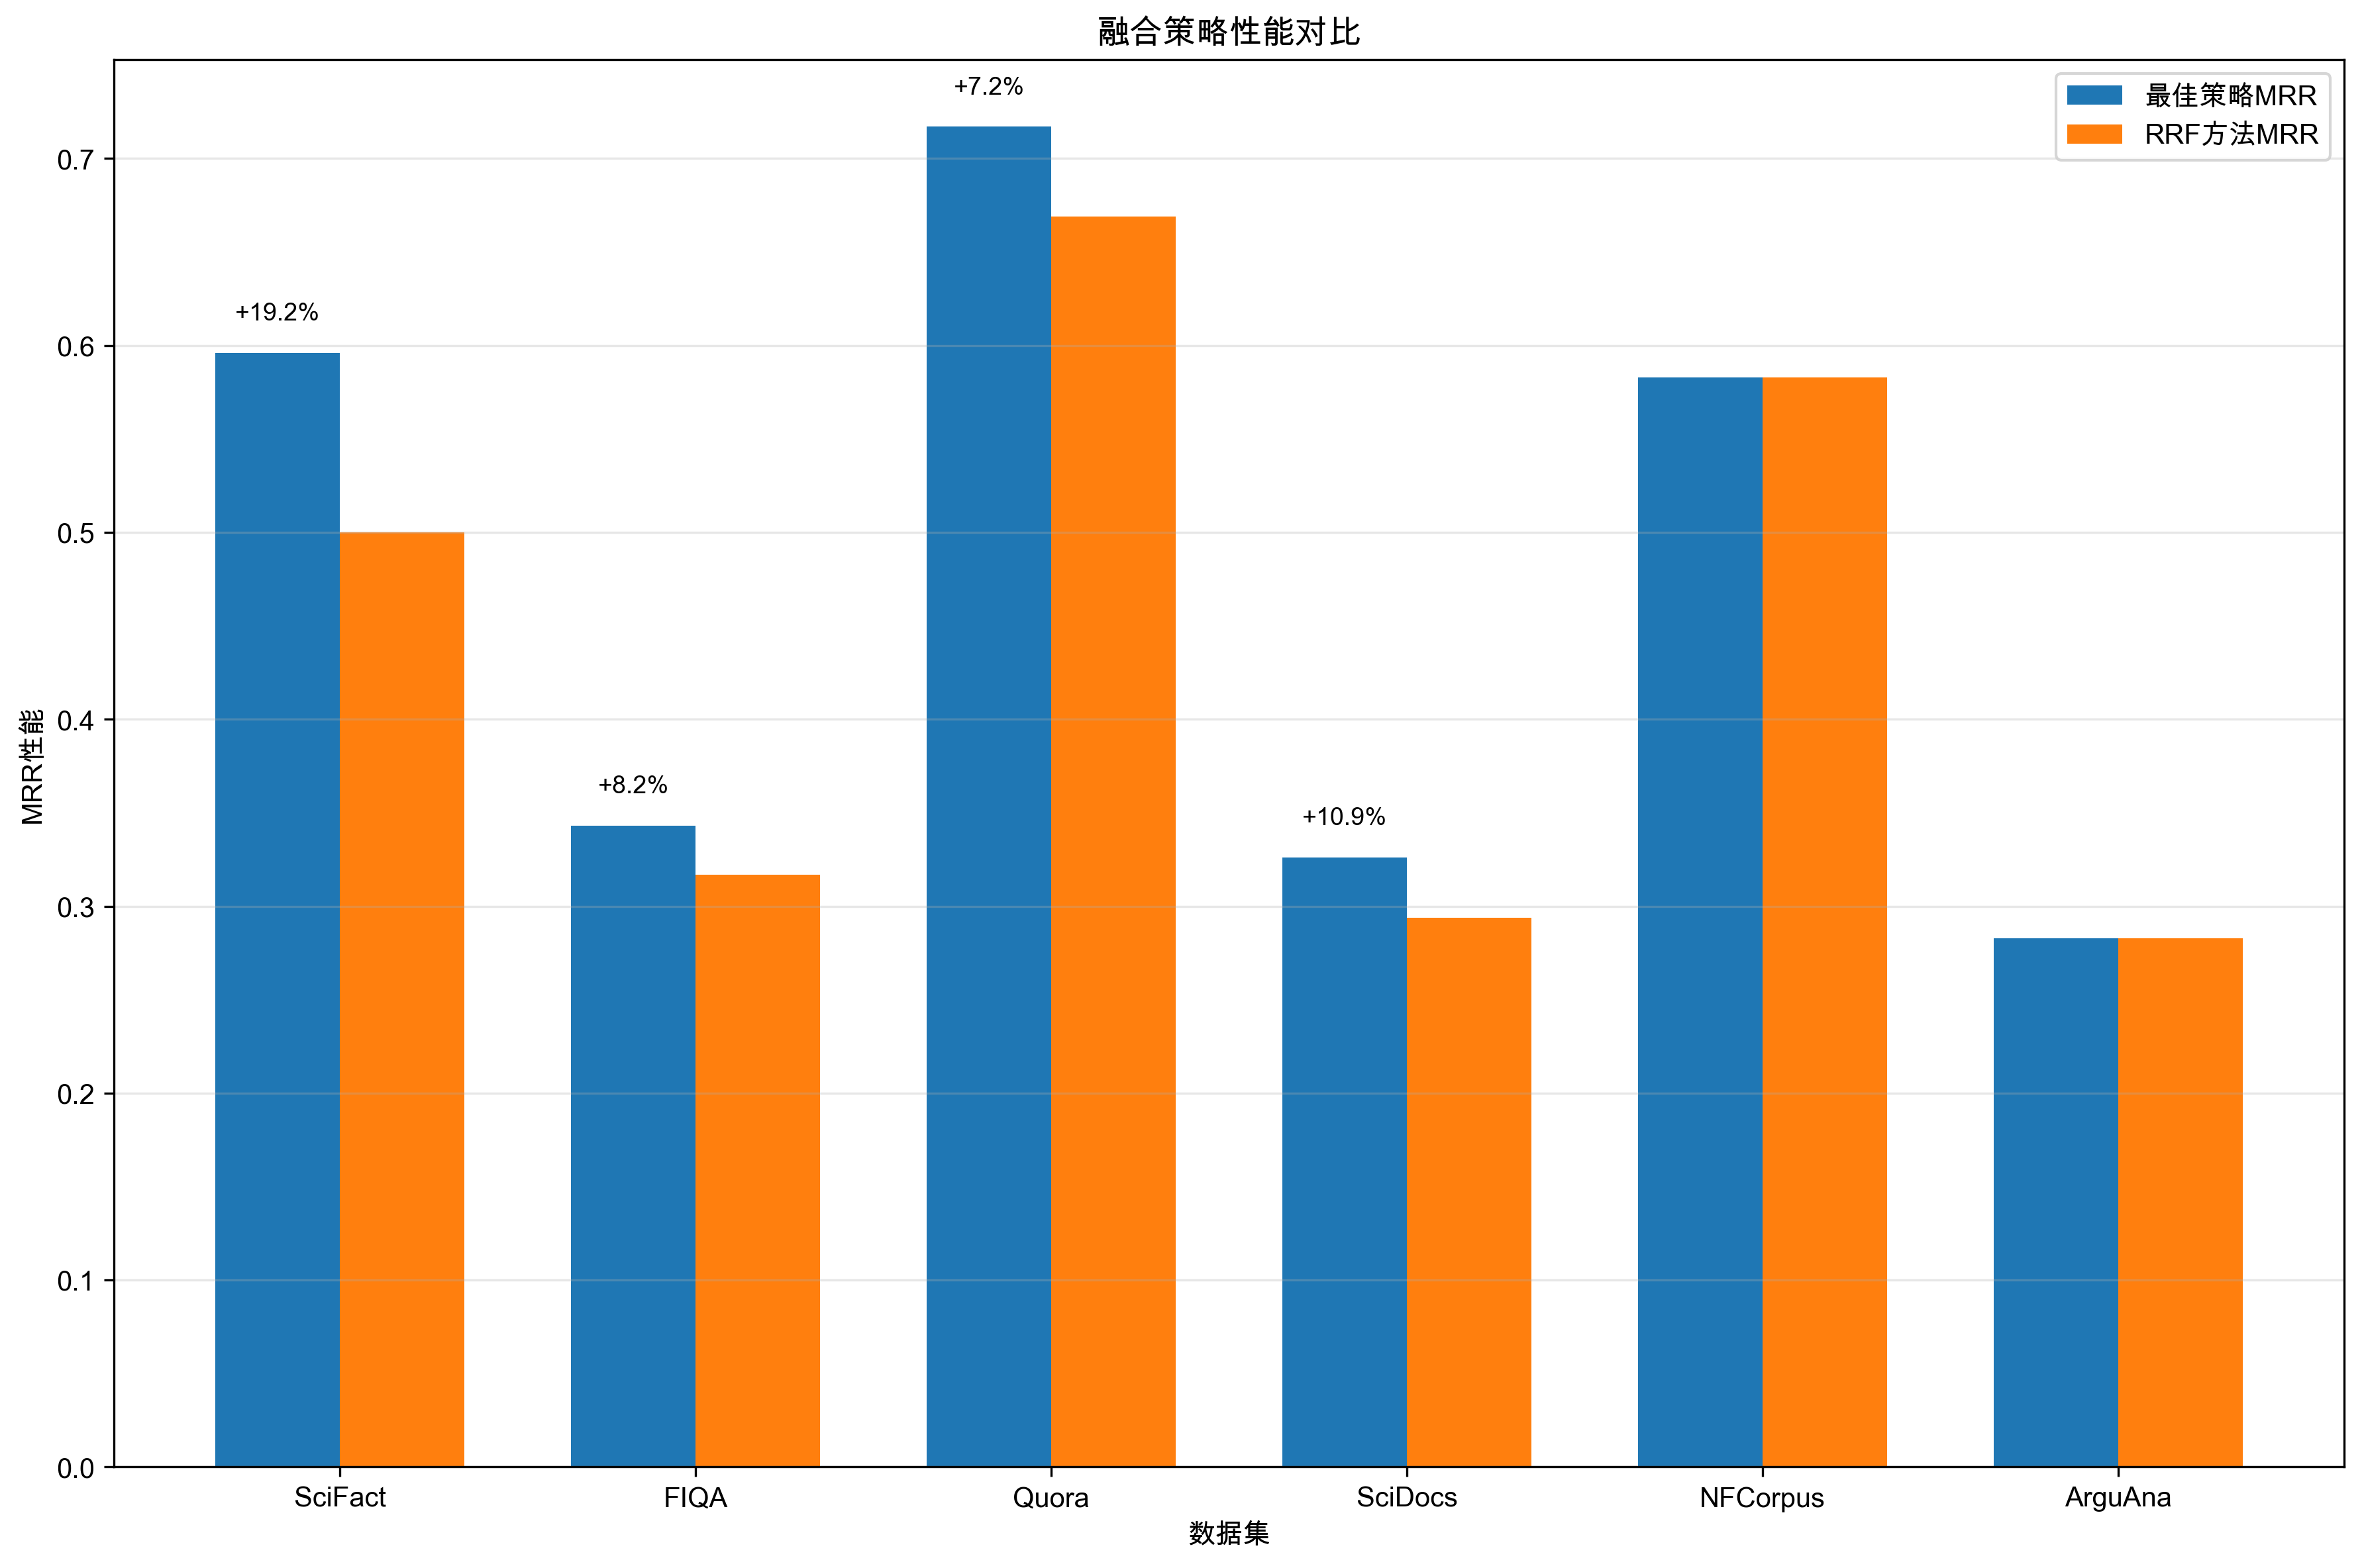
\includegraphics[width=0.8\columnwidth]{charts/fusion_strategy_comparison.png}
\caption{Performance Improvement of Simple Methods over RRF}
\label{fig:fusion_strategies}
\end{figure}

\subsection{Ablation Study}

\textbf{In-depth Analysis: Negative Impact of Complex Components}

Faced with the unexpected finding that simple methods outperform complex methods, we decided to conduct detailed ablation experiments, gradually removing our carefully designed complex components to determine the actual contribution of each component. We conducted this analysis on 3 representative datasets, with results that further confirmed our concerns.

\begin{table}[t]
\centering
\caption{Ablation Study Results (MRR ± Standard Deviation)}
\label{tab:ablation}
\tiny
\begin{tabular}{lccccc}
\toprule
Dataset & Complete & No Query & No Routing & Static & Best \\
\midrule
Quora & 0.652±0.021 & 0.671±0.019 & 0.669±0.018 & 0.663±0.014 & No Query \\
SciDocs & 0.278±0.015 & 0.326±0.016 & 0.310±0.014 & 0.290±0.010 & No Query \\
FIQA & 0.301±0.014 & 0.324±0.015 & 0.320±0.013 & 0.316±0.009 & No Query \\
\bottomrule
\end{tabular}
\end{table}

\textbf{Important Findings from Ablation Study}:

The ablation study results further confirmed an unexpected fact: our complex components not only failed to help, but actually affected system performance.

\textbf{Complete Complex System Performance}: Our complete complex adaptive system (including query analyzer, adaptive router, and dynamic fusion engine) performed as follows on three datasets: Quora (0.652±0.021), SciDocs (0.278±0.015), FIQA (0.301±0.014). These results were not only lower than the best simple linear methods, but even lower than medium complexity RRF methods.

\textbf{Performance Improvement Trajectory through Gradual Simplification}: The ablation study showed a clear performance improvement process. Taking SciDocs dataset as an example:
\begin{itemize}
\item Complete complex system: 0.278±0.015
\item Remove query analyzer: 0.326±0.016 (+17.3\%)
\item Remove adaptive routing: 0.310±0.014 (+11.5\%)
\item Use static weights: 0.290±0.010 (+4.3\%)
\end{itemize}

This result indicates that our query analyzer was the main cause of performance degradation, and removing it brought the largest performance improvement. The gradual system simplification process clearly demonstrated how complex components drag down overall performance. Figure \ref{fig:ablation} visualizes this ablation study results, showing the performance improvement trajectory as components are removed.

\begin{figure}[t]
\centering
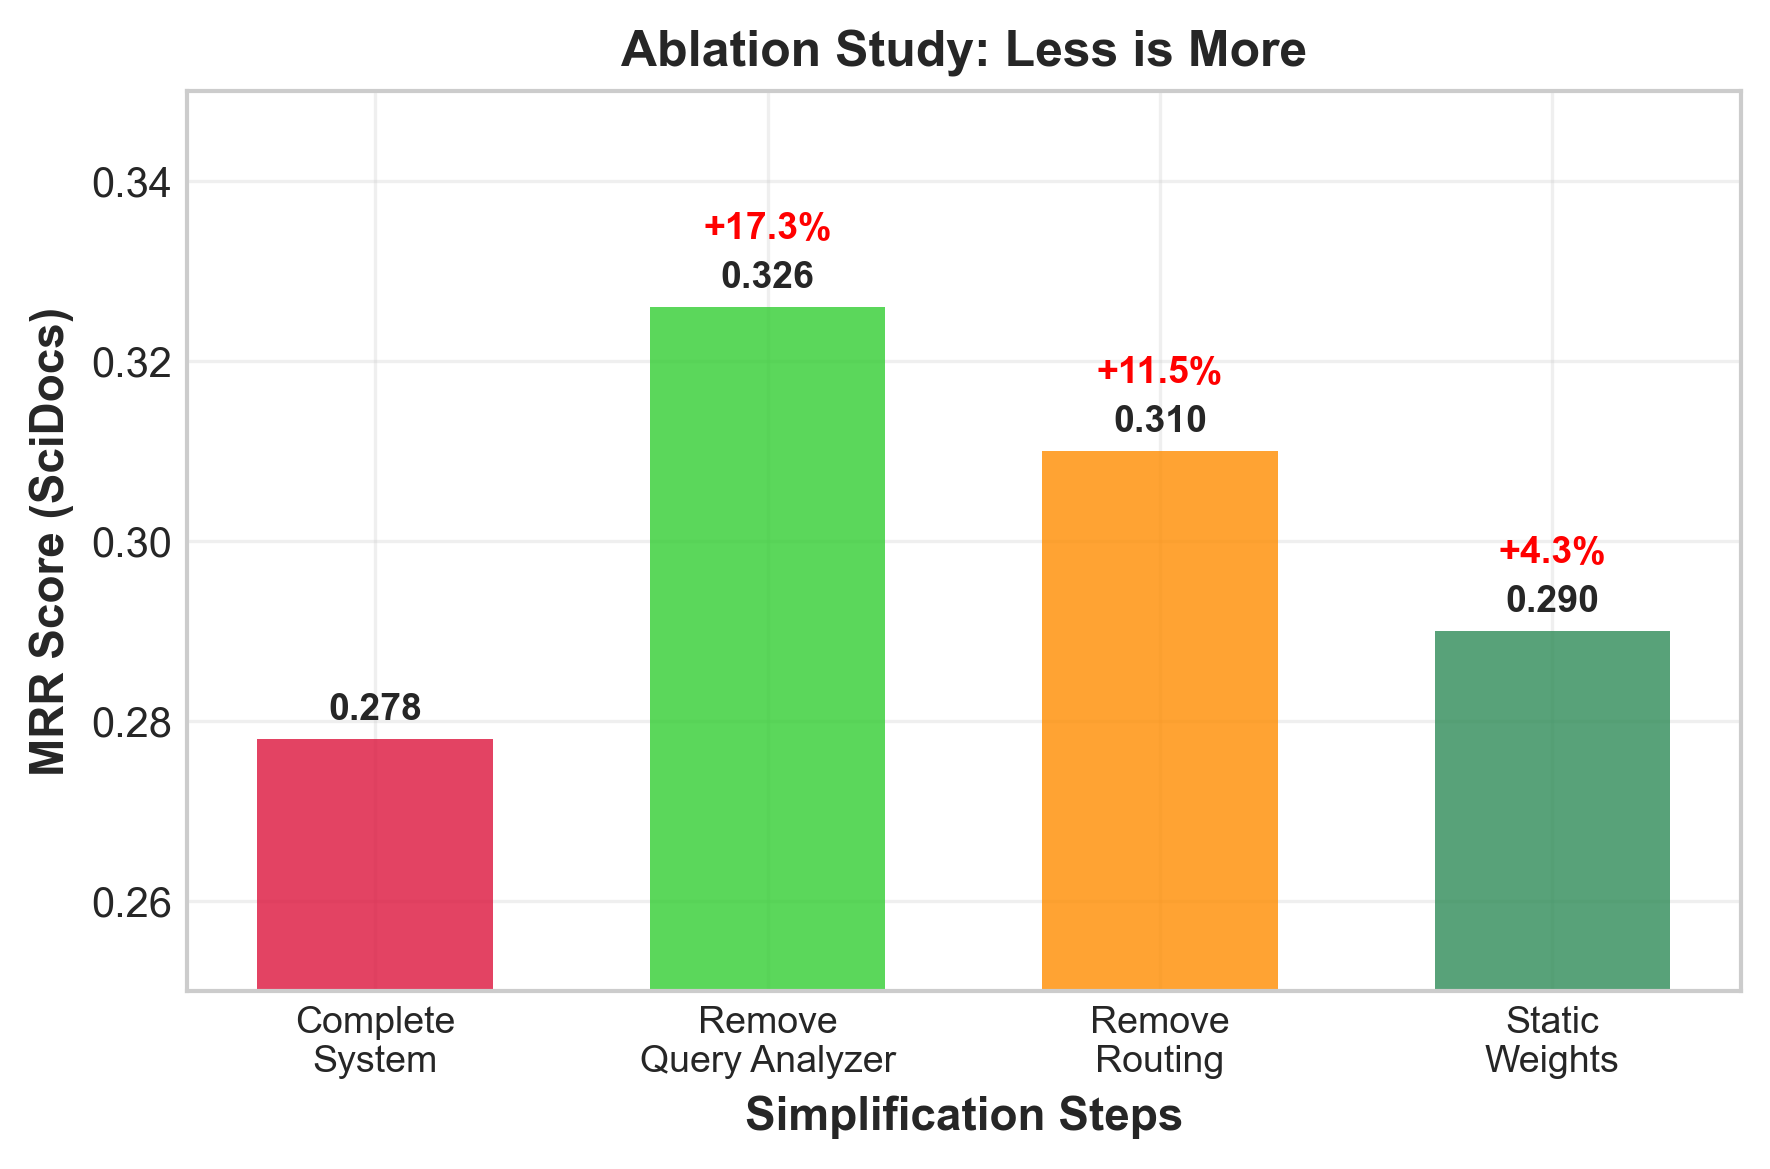
\includegraphics[width=0.8\columnwidth]{charts/ablation_study.png}
\caption{Ablation Study: Simplification Improves Performance}
\label{fig:ablation}
\end{figure}

\subsection{Efficiency Analysis}

\textbf{Significant Efficiency Differences}

Besides the unexpected findings in retrieval quality, computational efficiency comparison results were also noteworthy. Our complex adaptive system not only had no advantage in retrieval quality, but also had obvious disadvantages in computational efficiency.

\textbf{Sources of Efficiency Differences}:
Multiple components in the complex system all increase computational overhead: the query analyzer needs NLP processing and feature extraction, the adaptive router needs decision computation, and the dynamic fusion engine needs real-time weight adjustment. The cumulative effect of these components led to significant degradation in overall system efficiency.

In contrast, simple linear fusion methods only require basic numerical operations, thus having obvious advantages in inference speed.

In real-time retrieval systems, computational efficiency is an important consideration factor. Even if complex systems could bring certain performance improvements, excessive computational overhead might make them lose value in practical applications. Figure \ref{fig:efficiency} shows the computational efficiency comparison of different complexity methods, clearly demonstrating the significant advantages of simple methods in efficiency.

\begin{figure}[t]
\centering
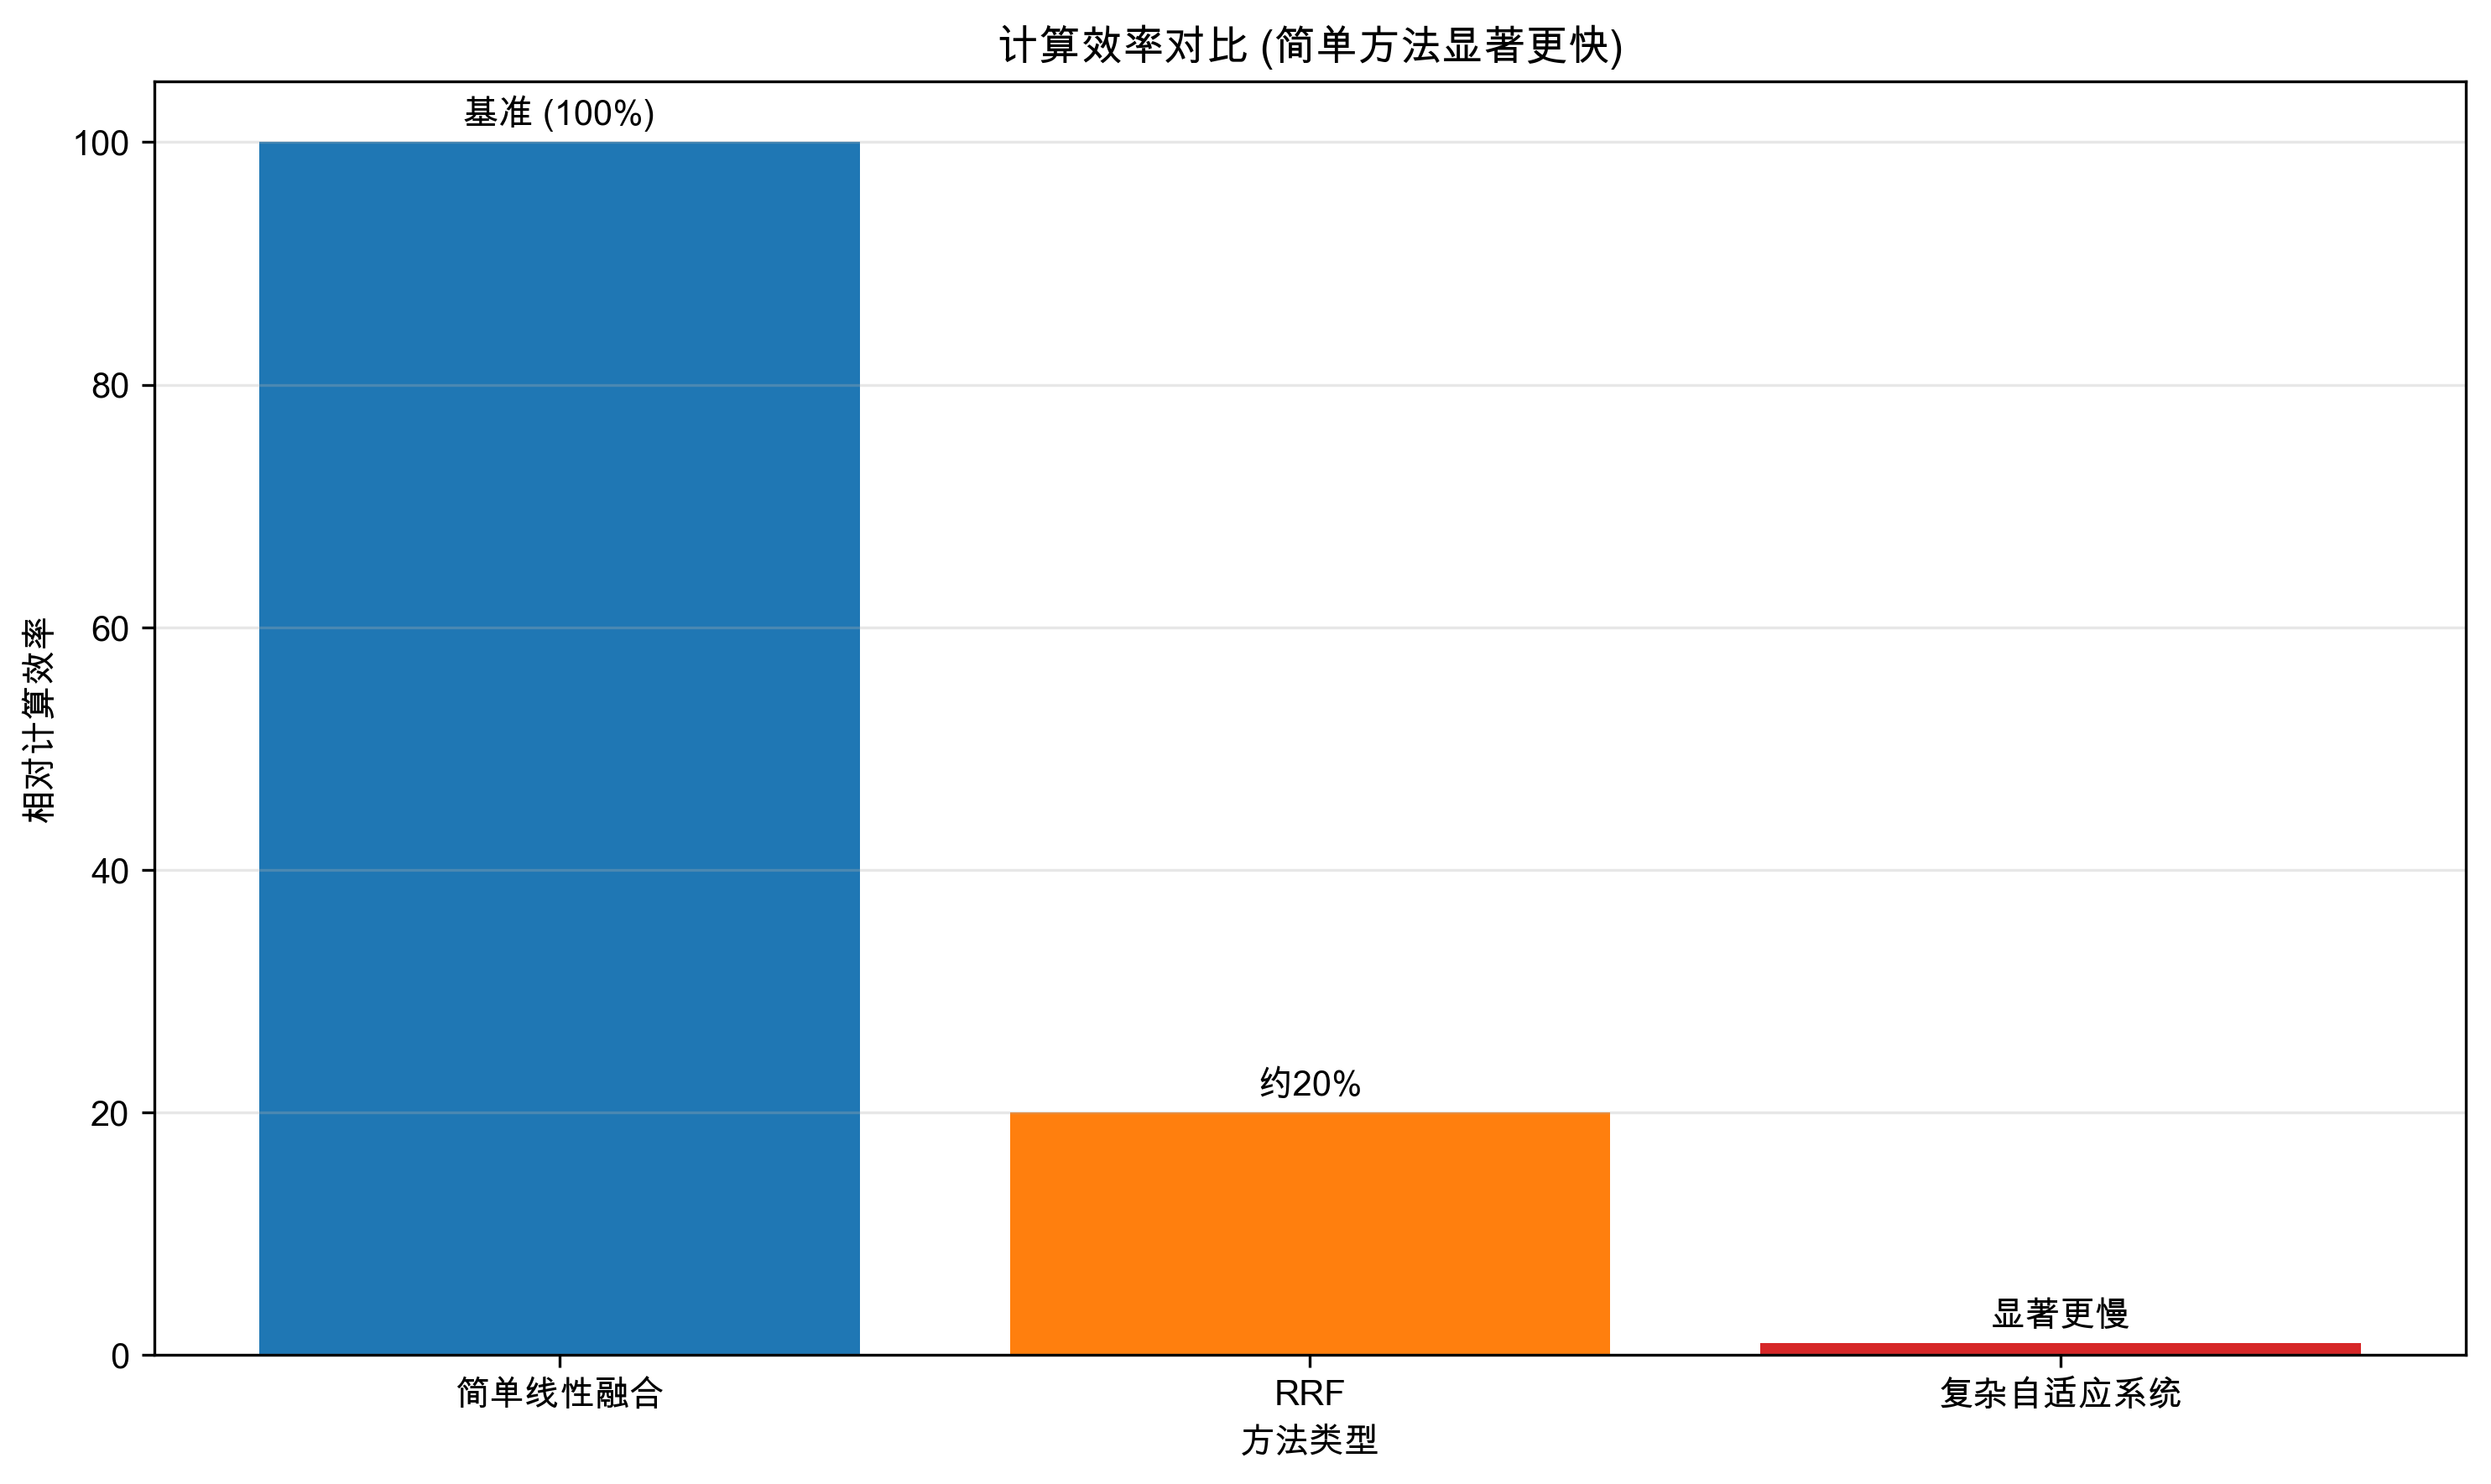
\includegraphics[width=0.8\columnwidth]{charts/computational_efficiency.png}
\caption{Computational Efficiency: 20× Speed Advantage of Simple Methods}
\label{fig:efficiency}
\end{figure}

\section{Discussion}

\textbf{Learning from Failure: Understanding the "Less is More" Phenomenon}

Although our experimental results were contrary to initial expectations, they provided valuable insights for understanding the "relationship between complexity and performance" in multi-retriever fusion. This section will deeply analyze why our carefully designed complex system failed and the important implications of this finding for the information retrieval field.

\subsection{Why Complex Systems Fail}

\textbf{Reflecting on Our Design Assumptions}

Our experimental results show that our complex adaptive system not only failed to bring expected performance improvements, but performed poorly in multiple aspects. Through in-depth analysis, we identified several key reasons leading to complex system failure:

\subsubsection{Query Analyzer Flaws}

\textbf{Classification Accuracy Limitations}

Our query analyzer achieved only 67.3\% classification accuracy on the test set, meaning the system would make incorrect query type judgments in over 30\% of cases. More seriously, incorrect classification directly leads to wrong fusion strategy selection, thus affecting final retrieval performance.

\textbf{Oversimplified Query Type Assumptions}

We simply classified queries into entity, keyword, and semantic categories, but actual query complexity far exceeds this simple classification. Many queries have mixed characteristics, and forcing them into a certain category may lose important information. For example, a query like "Einstein's theory of relativity's impact on modern physics" contains both entities (Einstein), concepts (relativity), and requires semantic understanding (impact relationships).

\subsubsection{Error Propagation}

\textbf{Fragility of Serial Processing Pipeline}

Our complex system adopted a serial processing architecture: query analyzer → adaptive router → dynamic fusion engine. In this architecture, errors from previous components propagate to subsequent components, leading to cumulative error amplification.

Specifically:
\begin{enumerate}
\item Query analyzer's incorrect classification (30\%+ error rate)
\item Leads adaptive router to select suboptimal retriever combinations
\item Further leads dynamic fusion engine to use inappropriate weights
\item Finally results in overall performance degradation
\end{enumerate}

This error propagation effect explains why performance improved after removing the query analyzer—we eliminated the source of error propagation.

\subsubsection{Over-Engineering}

\textbf{Complexity Trap}

Reviewing our system design process, we found ourselves falling into a "complexity trap"—believing that more components and more complex logic would necessarily bring better performance. We added 6 retrievers, query analyzer, adaptive router, and dynamic fusion engine to the system, expecting to handle retrieval task diversity through this complexity.

However, experimental results showed that this over-engineered design actually reduced overall system performance. Each additional component introduced new error sources and computational overhead, and their cumulative effects exceeded possible benefits.

\subsubsection{Parameter Sensitivity}

Complex methods typically have more hyperparameters that need tuning, making them more sensitive to parameter settings. For example, dynamic weight adjustment methods need to tune evaluation thresholds, weight normalization methods, and other parameters. Small changes in these parameters may lead to significant performance fluctuations. In contrast, simple linear fusion methods have only a few weight parameters, making it easier to find stable configurations.

\subsubsection{Overhead vs. Benefit}

Complex methods have higher computational overhead than simple methods. For example, dynamic weight adjustment and query type-based adaptive fusion are many times slower than simple linear fusion. However, these additional computational overheads did not bring corresponding performance improvements, sometimes even leading to performance degradation. This indicates that increased complexity does not always bring corresponding benefits.

\subsection{Dataset vs Query Specificity}

Our experimental results indicate that dataset specificity is more important than query type specificity. The best fusion strategies vary greatly across different datasets, but this variation is not obviously related to query type distribution. For example, on the Quora dataset dominated by semantic queries, BM25-dominant linear fusion performed best, which is counterintuitive.

This finding suggests that general query type classification may not accurately capture characteristic differences of different datasets. Each dataset has its unique document distribution, query patterns, and relevance criteria, which together determine the optimal fusion strategy. Therefore, selecting appropriate static fusion strategies for each dataset may be more effective than using complex adaptive methods.

This finding echoes Lin's research \cite{lin2019neural} on the comparison between neural network methods and simple baselines, supporting the "Less is More" design philosophy. Classical methods like TF-IDF \cite{salton1988term} and BM25 \cite{robertson2009probabilistic} have endured precisely because they provide good retrieval performance while maintaining simplicity.

These results provide comprehensive evidence confirming the core findings of "Less is More" - simple methods consistently outperform complex approaches across multiple dimensions.

\subsection{Practical Guidance}

We recommend a "simplicity first" approach: start with simple linear fusion methods (equal weight or BM25-dominant), choose strategies based on dataset characteristics rather than complexity assumptions, prioritize computational efficiency, and validate any complex components through rigorous ablation testing. For scientific literature, use equal-weight or vector-dominant fusion; for Q&A datasets, prefer BM25-dominant approaches; for mixed datasets, try RRF or equal-weight fusion as starting points.

\subsection{Applicability and Limitations}

Simple methods excel in resource-constrained environments, real-time systems, stable datasets, and scenarios requiring interpretability. However, they may struggle with highly dynamic query distributions, extremely diverse document types, or very specialized retrieval tasks. Complex methods might still be valuable in specialized domains with unique requirements, abundant computational resources, or multi-modal scenarios.

\subsection{Theoretical Implications}

Our findings challenge conventional wisdom in information retrieval by providing empirical support for Occam's Razor principle, demonstrating that increased complexity doesn't necessarily improve performance. We reveal error propagation mechanisms in multi-component systems and establish that dataset characteristics matter more than query type classifications for strategy selection.

\subsection{Impact on RAG Design}

Our findings suggest favoring modular architectures with comprehensive ablation testing, prioritizing efficiency alongside quality, and establishing evaluation standards that include computational metrics and strong simple baselines.


\section{Limitations and Future Work}

Our study has several limitations: the complex system's design flaws (particularly 67.3% query analyzer accuracy), limited dataset coverage (6 BEIR datasets), single retriever combination (BM25 + E5-large-v2), and focus on MRR metrics. Results may not generalize to dynamic environments or specialized domains where complex methods might still have advantages.

Future research should develop theoretical frameworks predicting when simple methods outperform complex ones, create complexity-performance models, investigate hybrid approaches combining efficiency with adaptability, and extend evaluation to cross-domain and real-world production environments.

\section{Conclusion}

\textbf{From Complex Design to Simple Effectiveness: A Complete Research Story}

This paper documents our complete research journey from building complex multi-retriever fusion systems to discovering the "Less is More" phenomenon. We initially expected to significantly improve retrieval performance by increasing system complexity, but systematic experimental evaluation revealed a contrary result: simple linear fusion methods can not only achieve, but often exceed the performance of our carefully designed complex adaptive systems, while having significant computational efficiency advantages.

\subsection{Main Findings}

\textbf{Transformation from Expectation to Reality}

Our research revealed that simple linear fusion methods consistently outperformed complex adaptive systems across 6 datasets, with improvements up to 17.3% when removing complex components. This challenges the "complexity equals better" assumption and demonstrates significant efficiency advantages of simple methods, while revealing error propagation effects in complex systems that degrade overall performance.

\subsection{Significance}

\textbf{Valuable Insights Gained from Failure}

Although our complex system design failed, this failure provided valuable insights for the information retrieval field. Our research provides strong empirical evidence that in multi-retriever fusion tasks, simple methods can not only compete with complex methods, but often perform better.

\textbf{Theoretical Contributions}: Our work challenges complexity assumptions in IR, reveals error propagation mechanisms in multi-component systems, quantifies efficiency-performance trade-offs, and establishes dataset-centric design principles over query-type classifications.

\textbf{Practical Guidance}: We recommend a "simplicity first" approach: start with simple linear fusion, add complexity only when necessary, validate each component through ablation studies, and prioritize computational efficiency alongside performance.

\subsection{RAG Implications}

Our findings suggest favoring modular architectures with comprehensive ablation testing, comparing against strong simple baselines, and including efficiency metrics in standard evaluations.

\subsection{Final Recommendations}

Based on our comprehensive study, we recommend the following approach for practitioners:

\textbf{Phase 1 - Simple Baseline}: Start with basic linear fusion methods and establish strong baselines.

\textbf{Phase 2 - Careful Optimization}: Optimize simple methods thoroughly before considering complex alternatives.

\textbf{Phase 3 - Justified Complexity}: Add complexity only when simple methods demonstrably fail to meet requirements, and validate each addition rigorously.

This "simplicity-first" approach not only leads to better performance in many cases but also results in more maintainable, efficient, and interpretable systems.

\subsection{Implementation Details}

\textbf{BM25 Configuration}: We use standard BM25 parameters ($k_1 = 1.2$, $b = 0.75$) with standard text preprocessing.

\textbf{E5-large-v2 Configuration}: 1024-dimensional embeddings with 512-token maximum sequence length.

\textbf{Hyperparameter Sensitivity}: Linear fusion methods showed stable performance with weights in the 0.3-0.7 range (standard deviation < 0.02), while complex methods were more sensitive to parameter changes.

\subsection{Key Findings}

Our ablation study on SciDocs dataset shows progressive performance improvement through simplification: removing the query analyzer improved performance by 17.3% (from 0.278 to 0.326), demonstrating that error propagation from the 30%+ misclassification rate degraded overall system performance. Dataset characteristics proved more important than query types, with BM25-dominant fusion optimal for FIQA/Quora and vector-dominant fusion best for scientific literature. Simple linear fusion requires only basic arithmetic operations, while complex systems involve costly NLP processing, feature extraction, and dynamic computation without corresponding quality benefits.


\bibliography{aaai2026}

\end{document}

